\documentclass{article}
\usepackage{graphicx}
\usepackage{listings}
\usepackage{ctex}
\usepackage{graphicx}
\usepackage[a4paper, body={18cm,22cm}]{geometry}
\usepackage{amsmath,amssymb,amstext,wasysym,enumerate,graphicx}
\usepackage{float,abstract,booktabs,indentfirst,amsmath}
\usepackage{array}
\usepackage{booktabs} %调整表格线与上下内容的间隔
\usepackage{multirow}
\usepackage{diagbox}
\usepackage{indentfirst}
\usepackage{bm}
\usepackage{fancyhdr}




\pagestyle{fancy}

\lhead{\bfseries \normalsize 学号:1952033\quad 姓名:侯雅玥 \quad 组员:廖宏 \\实验名称:触发器基本功能测试实验\quad 课程名称:电子技术实验\quad 专业:微电子科学与工程 } 
\rhead{}

\begin{document}
	\section{\zihao{4} 实验名称:触发器基本功能测试实验}
    \section{\zihao{4} 实验目的}
    \zihao {5} (1)学习触发器逻辑功能的测试方法。\par
               (2)了解基本 RS触发器、D触发器及IK触发器的逻辑功能及触发方式。\par 
               (3)进一步学习用示波器测量比较两路相关信号波形的周期、脉宽等参数的方法。 \par 
 
   	\section{\zihao{4} 实验原理}
       双稳态触发器具有两个互补的输出端Q和Q',触发器正常工作时,Q与Q'的逻辑电平总是互补,即一个为"0"时另一个一定是"1"。(当触发器工作在非正常状态时,Q和Q'的输出电平有可能相同,使用时必须注意避免出现这种情况)。
       RS触发器具有两个开关量特性的激励输入端R和S,R的有效电平使触发器复位(Reset),Q="0";S的有效电平使触发器置位(Set),Q="1",所以称为Reset Set 触发器。
       图1是两个与非门互相反馈组成的基本 RS
       触发器电路。当激励 S为有效电平时,输出 Q 立即置位为"1",而激励 R 为有效电平时,输出 Q 复位为
       "0",两者都为无效电平时,输 出保持原来的状态不变。\par
       JK 触发器具有两个激励输入端 J 和 K,其特性
       方程为∶$Q_{n+1}=JQ_n'+K'Q_n$。在有效时钟脉冲触发时,
       可以实现"同步置位"、"同步复位"、"状态不变"、"状
       态变反"四种功能。74LS112是下降沿触发有效的集成双JK触发器,片上有两个JK触发器,引脚标号以"1"和"2"区别,如图 2所示。\par
       \begin{figure}[h]
        \begin{minipage}[t]{0.5\linewidth} % 如果一行放2个图,用0.5,如果3个图,用0.33  
          \centering   
          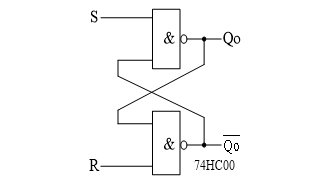
\includegraphics[width=2.8in]{H:/电子技术试验/4-20/4-20-1.png}   
          \caption{与非门互相反馈组成的基本RS}   
          \label{fig:side:a}   
        \end{minipage}%   
        \begin{minipage}[t]{0.5\linewidth}   
          \centering   
          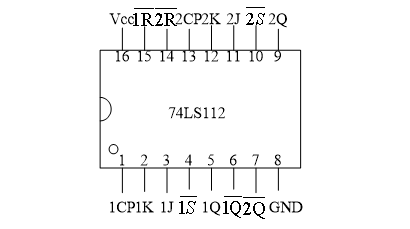
\includegraphics[width=2.8in]{H:/电子技术试验/4-20/4-20-2.png}   
          \caption{74LS112引脚图}   
          \label{fig:side:b}   
        \end{minipage}   
      \end{figure}
      \par
       D触发器只有一个激励输入端 D。当触发脉冲有效时,D触发器的输出与激励输入相同,由于在时间上滞后于输入,所以又称 Delay触发器。74LS74是上升沿触发有效的双 D集成触发器,片上有两个D触发器,引脚排列如图3所示。
       集成触发器一般具有直接(Direct)置位、复位控制端S。与R,如74LSI12和74LS74引脚图所示。当R,或S,有效时(为低电平"0"),触发器立即被
     
      复位或者置位。所以 $R_D$与$S_D$又称异步复位、置位端。直接置位、复位可以用来判断预置触发器的初始状态,但在使用时必须注意两者不允许同时有效,而不允许与时钟触发控制同时有效。
T触发器也只有一个激励控制端T,其特 
性方程为$Q_{n+1}=JQ_n'+K'Q_n$当触发条件满

足时,若激励T="0",触发器的状态不变,当
T="1",触发器的状态变反。
\begin{figure}[h]
    \begin{minipage}[t]{0.5\linewidth} % 如果一行放2个图,用0.5,如果3个图,用0.33  
      \centering   
      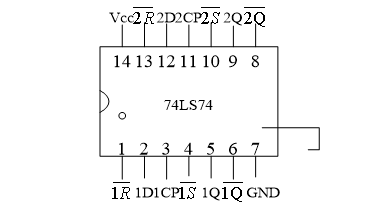
\includegraphics[width=2.8in]{H:/电子技术试验/4-20/4-20-3.png}   
      \caption{$I_{EH}$}   
      \label{fig:side:a}   
    \end{minipage}%   
    \begin{minipage}[t]{0.5\linewidth}   
      \centering   
      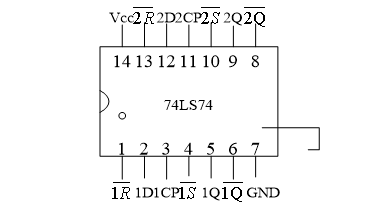
\includegraphics[width=2.8in]{H:/电子技术试验/4-20/4-20-3.png}   
      \caption{$N_o$}   
      \label{fig:side:b}   
    \end{minipage}   
  \end{figure}
\par
T'触发器没有激励输入,只受触发时钟脉 ce风SLSL
冲控制,其特性方程为$Q_{n+1}=Q_n'$只要触发
条件满足,T′触发器状态的输出状态随触发脉
冲CP输入连续翻转。如果T触发器的初
状态为"0",奇数个触发脉冲输入后其状态为
"1",偶数个触发脉冲输入后状态为"O",类似
l位二进制数累计触发脉冲输入的个数(进
位溢出不计)。\par
图5中两个JK触发器构成了下降沿有效的 T'触发器(J=K="1"),状态方程为$Q_{n+1}=Q_n'$;,具有的计数特性。FFO 的触发脉冲为 CP,$Q_0$在每个CP 脉冲下降沿时刻状态变反;FF1的时钟是FFO 的输出$Q_0'$,所以 FF1在 $Q_0$上升沿(Q的下降沿)时刻状态变反。$Q_0$与$Q_1$的输出波形如图 6所示。
由信号波形可见,在每个时钟脉冲下降沿后,$Q_0$与$Q_1$的状态码按"00"-"11'- "10"-“01"-"00"的规律循环变化,循环周期为 4个时钟脉冲周期。状态变化是以2位二进制码递减方式累计输入时钟脉冲的个数,电路功能为2位异步二进制减计数器。\par 
一般,用n个T'触发器可以构成双位异步二进制计数器。除最低位触发器直接由时钟CP控制外,其他各触发器的时钟都由相邻低位的状态输出控制。

      \begin{figure}[h]
        \begin{minipage}[t]{0.5\linewidth} % 如果一行放2个图,用0.5,如果3个图,用0.33  
          \centering   
          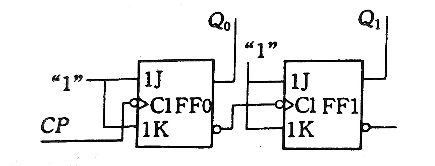
\includegraphics[width=2.8in]{H:/电子技术试验/4-20/4-20-5.png}   
          \caption{$I_{EH}$}   
          \label{fig:side:a}   
        \end{minipage}%   
        \begin{minipage}[t]{0.5\linewidth}   
          \centering   
          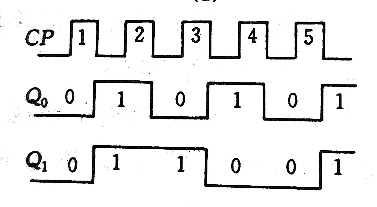
\includegraphics[width=2.8in]{H:/电子技术试验/4-20/4-20-6.png}   
          \caption{$N_o$}   
          \label{fig:side:b}   
        \end{minipage}   
      \end{figure}
       



\newpage
\section{\zihao{4} 实验电路}
\begin{figure}[h]
    %\small
    \centering
    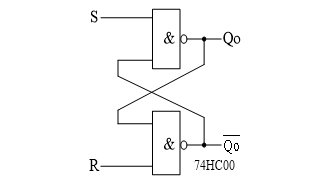
\includegraphics[width=3in]{H:/电子技术试验/4-20/4-20-1.png}
    \caption{RS触发器 } \label{fig:aa}
  \end{figure}
\begin{figure}[h]
  %\small
  \centering
  
\includegraphics[width=3.5in]{H:/电子技术试验/4-20/4-20-7.png}
  \caption{集成触发器实验电路} \label{fig:aa}
\end{figure}
\begin{figure}[h]
  %\small
  \centering
  
\includegraphics[width=3.5in]{H:/电子技术试验/4-20/4-20-8.png}
  \caption{信号传输电路} \label{fig:aa}
  \end{figure}

\newpage

\section{\zihao{4} 实验内容及步骤}
1.基本RS触发器功能测试:按图7接线,验证RS触发器的基本逻辑功能,填入表1\par
2.集成JK触发器功能测试:验证集成JK触发器功能,填入表2,表3\par
3.集成触发器应用:按图8接线,电路的时钟CP输入1kHz脉冲波,用示波器观测和记录CP,Q1,Q2的波形。\par
4.信号传输中的竞争冒险现象观察:按图4-1-5接线,用示波器观察并记录A,B,C 波形。\par



\section{\zihao{4} 数据及误差处理}
\subsection{与门基本RS触发器的逻辑功能测试}
\begin{table}[h]
    \centering  
    \begin{tabular}{c|c|c|c|c}
        \hline
              R             & S    &$Q_0$    &$Q_0'$             &功能  \\ \hline
              0             & 1    &0        &   1             & 置"0" \\ \hline
              1             & 1    &0        &   1               & 保持            \\ \hline
              1             & 0    &1        &   0              & 置"0"            \\ \hline
              1             & 1    &1        &   0               & 保持            \\ \hline
              0             & 0    &/        &   /               & 禁止(不定)            \\ \hline
              1             & 1    &/        &   /              & 保持            \\ \hline
        
            \end{tabular}
  \end{table}


\subsection{集成JK触发器的直接置位复位功能测试}
\begin{table}[h]
    \centering  
    \begin{tabular}{c|c|c|c|c}
        \hline
              R             & S    &$Q_0$    &$Q_0'$             &功能  \\ \hline
              0             & 1    &0   & 1                      & 置"0" \\ \hline
              1             & 1    &0        &   1              & 保持            \\ \hline
              1             & 0    &1        &   0               & 置"0"            \\ \hline
              1             & 1    &1        &   0               & 保持            \\ \hline
              0             & 0    &1        &   1               & 禁止(不定)            \\ \hline
              1             & 1    &1        &   0               & 保持            \\ \hline
        
            \end{tabular}
  \end{table}

\newpage
  \subsection{集成JK触发器的激励功能测试}
\begin{table}[h]
  \centering  
  \begin{tabular}{c|c|c|c|c|c|c|c|c|c|c}
      \hline
            J  &1         &1          &0        &0          &0        &0         &1         &1          &1        &1   \\ \hline
            K  &0         &0          &0        &0          &1        &1         &1         &1          &1        &1    \\ \hline
            CP &$\uparrow$  &$\downarrow$ &$\uparrow $&$\downarrow$ &$\uparrow$ &$\downarrow$ &$\uparrow$ &$\downarrow $&$\uparrow $&$\downarrow$     \\ \hline
            Q  &0         &1          &1        &1          &1        &0         &0         &1          &1        &0   \\ \hline
            Q' &1         &0          &0        &0          &0        &1         &1         &0          &0        &1    \\ \hline
          \end{tabular}
 \end{table}

 \subsection{集成触发器应用}
 \begin{figure}[h]
  \begin{minipage}[t]{0.5\linewidth} % 如果一行放2个图,用0.5,如果3个图,用0.33  
    \centering   
    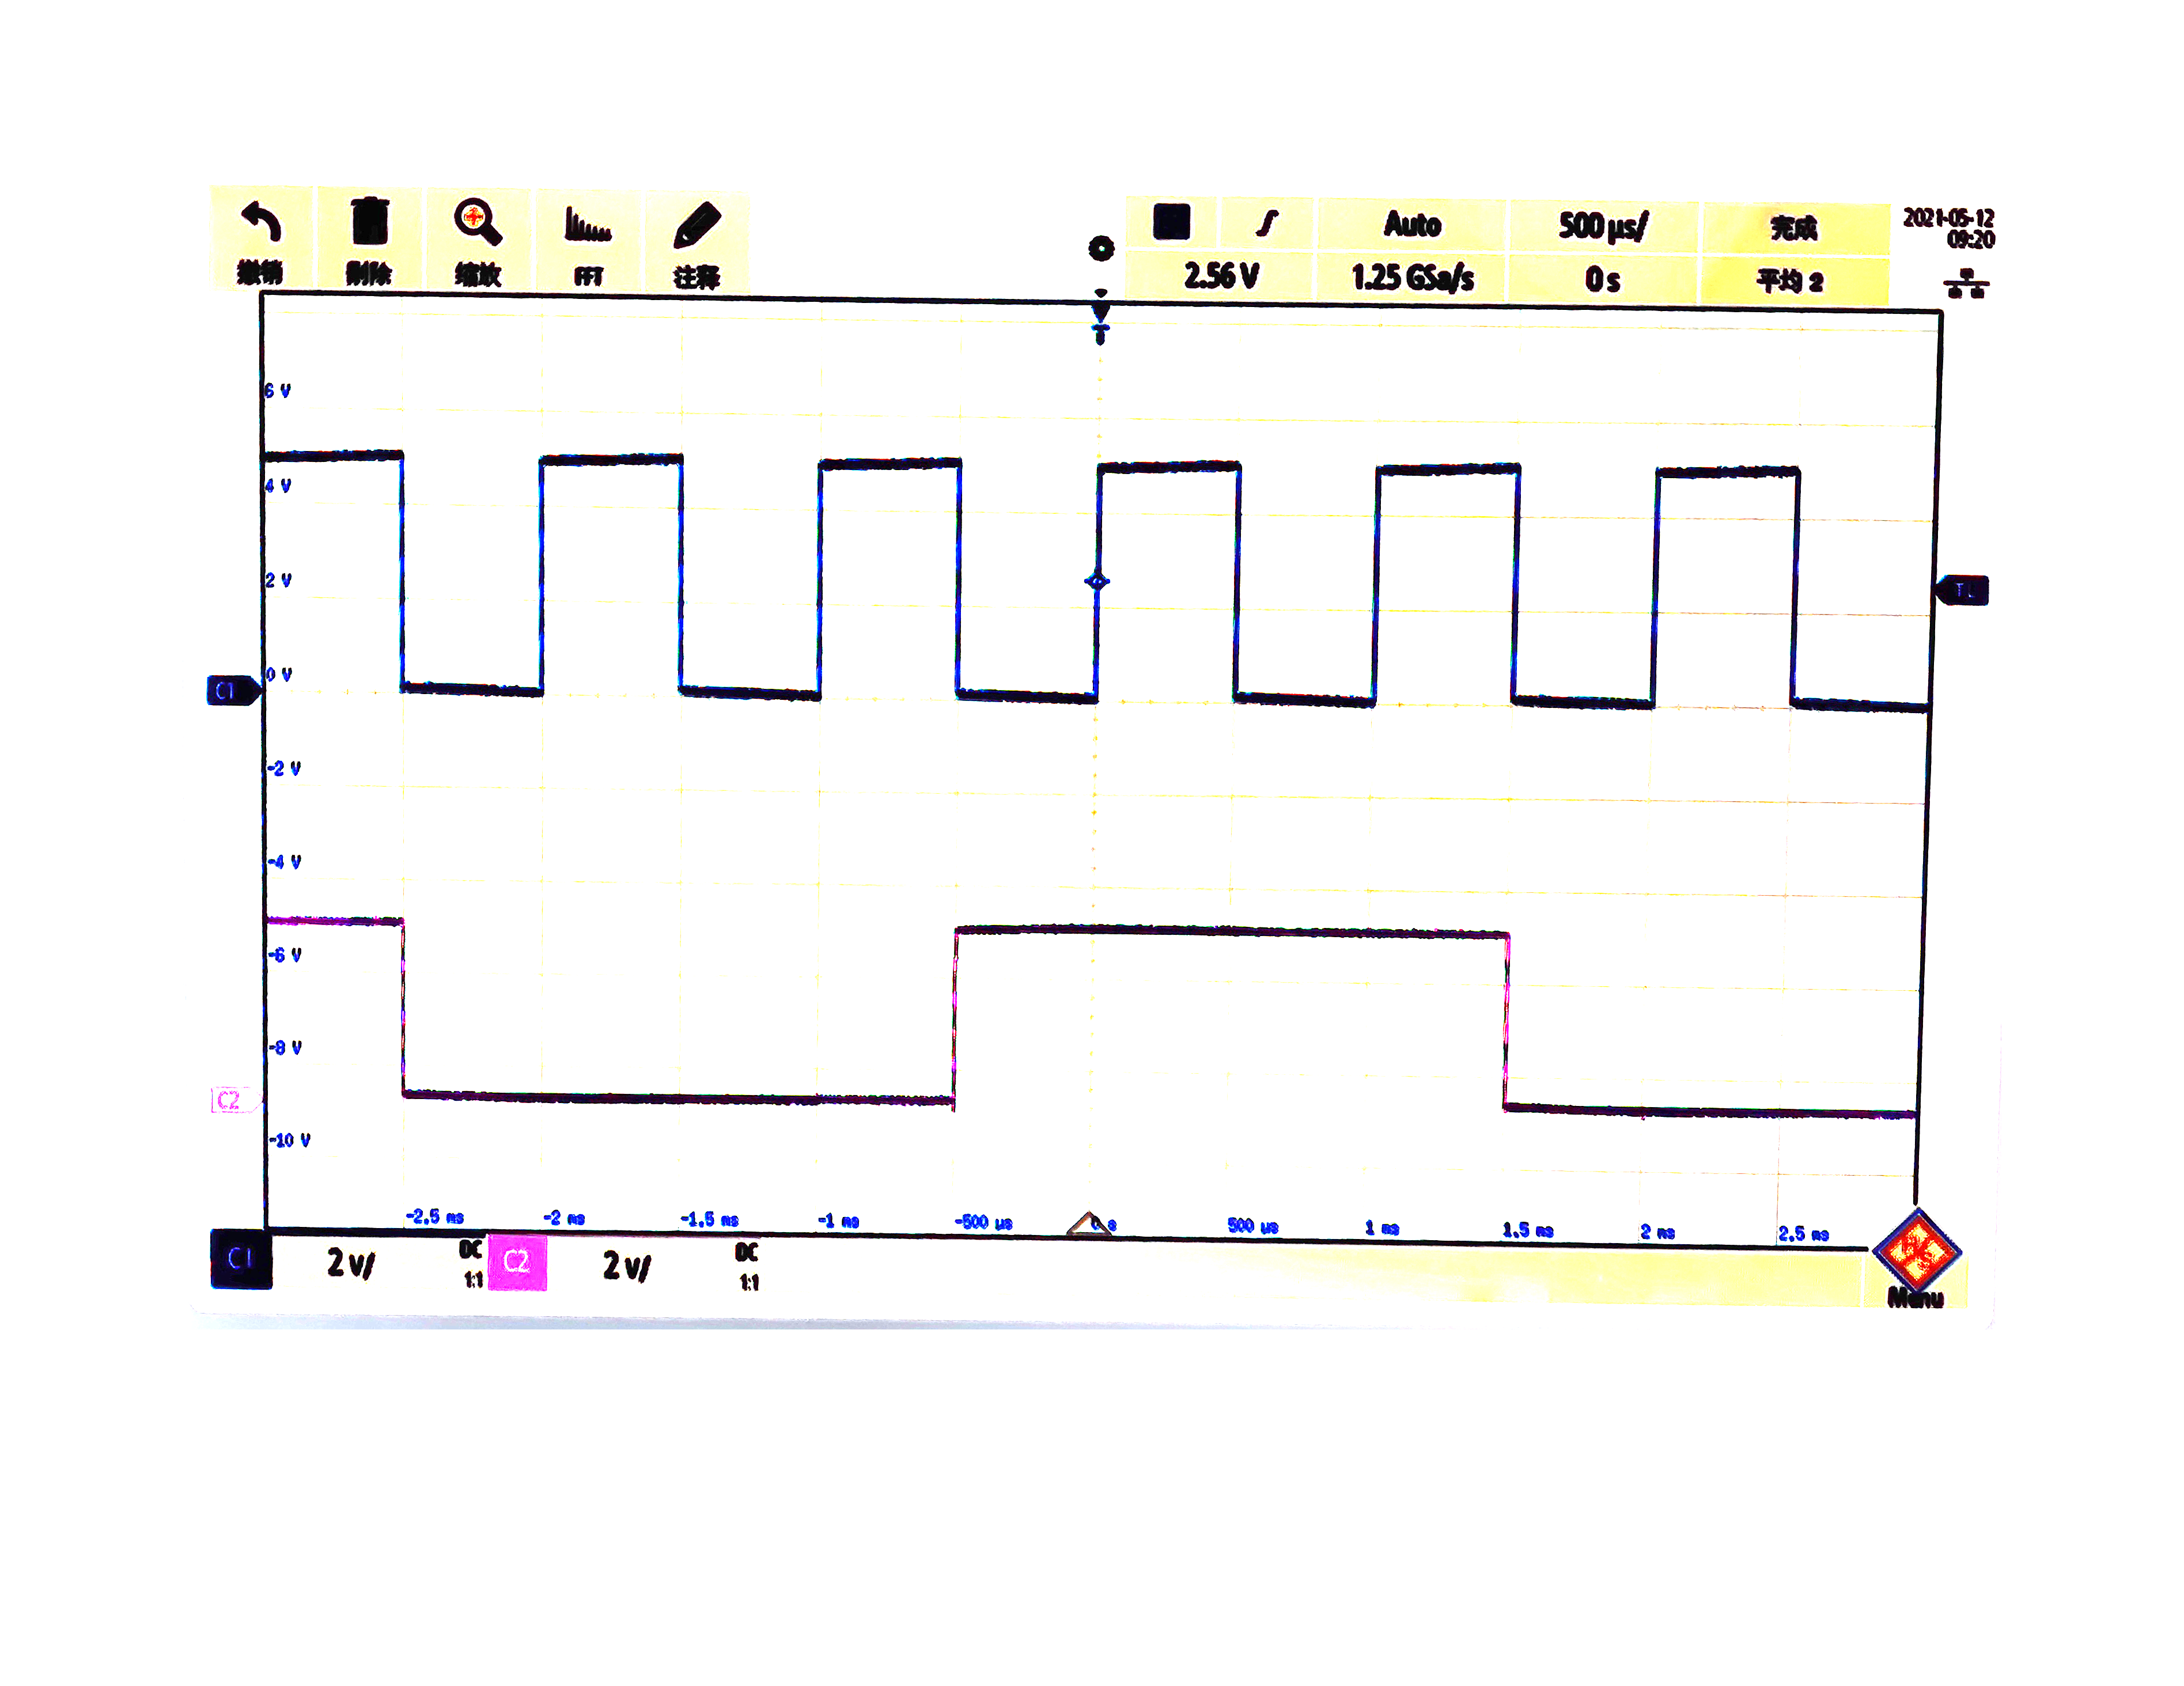
\includegraphics[width=2.8in]{H:/电子技术试验/4-20/4-20-9.png}   
    \caption{$I_{EH}$}   
    \label{fig:side:a}   
  \end{minipage}%   
  \begin{minipage}[t]{0.5\linewidth}   
    \centering   
    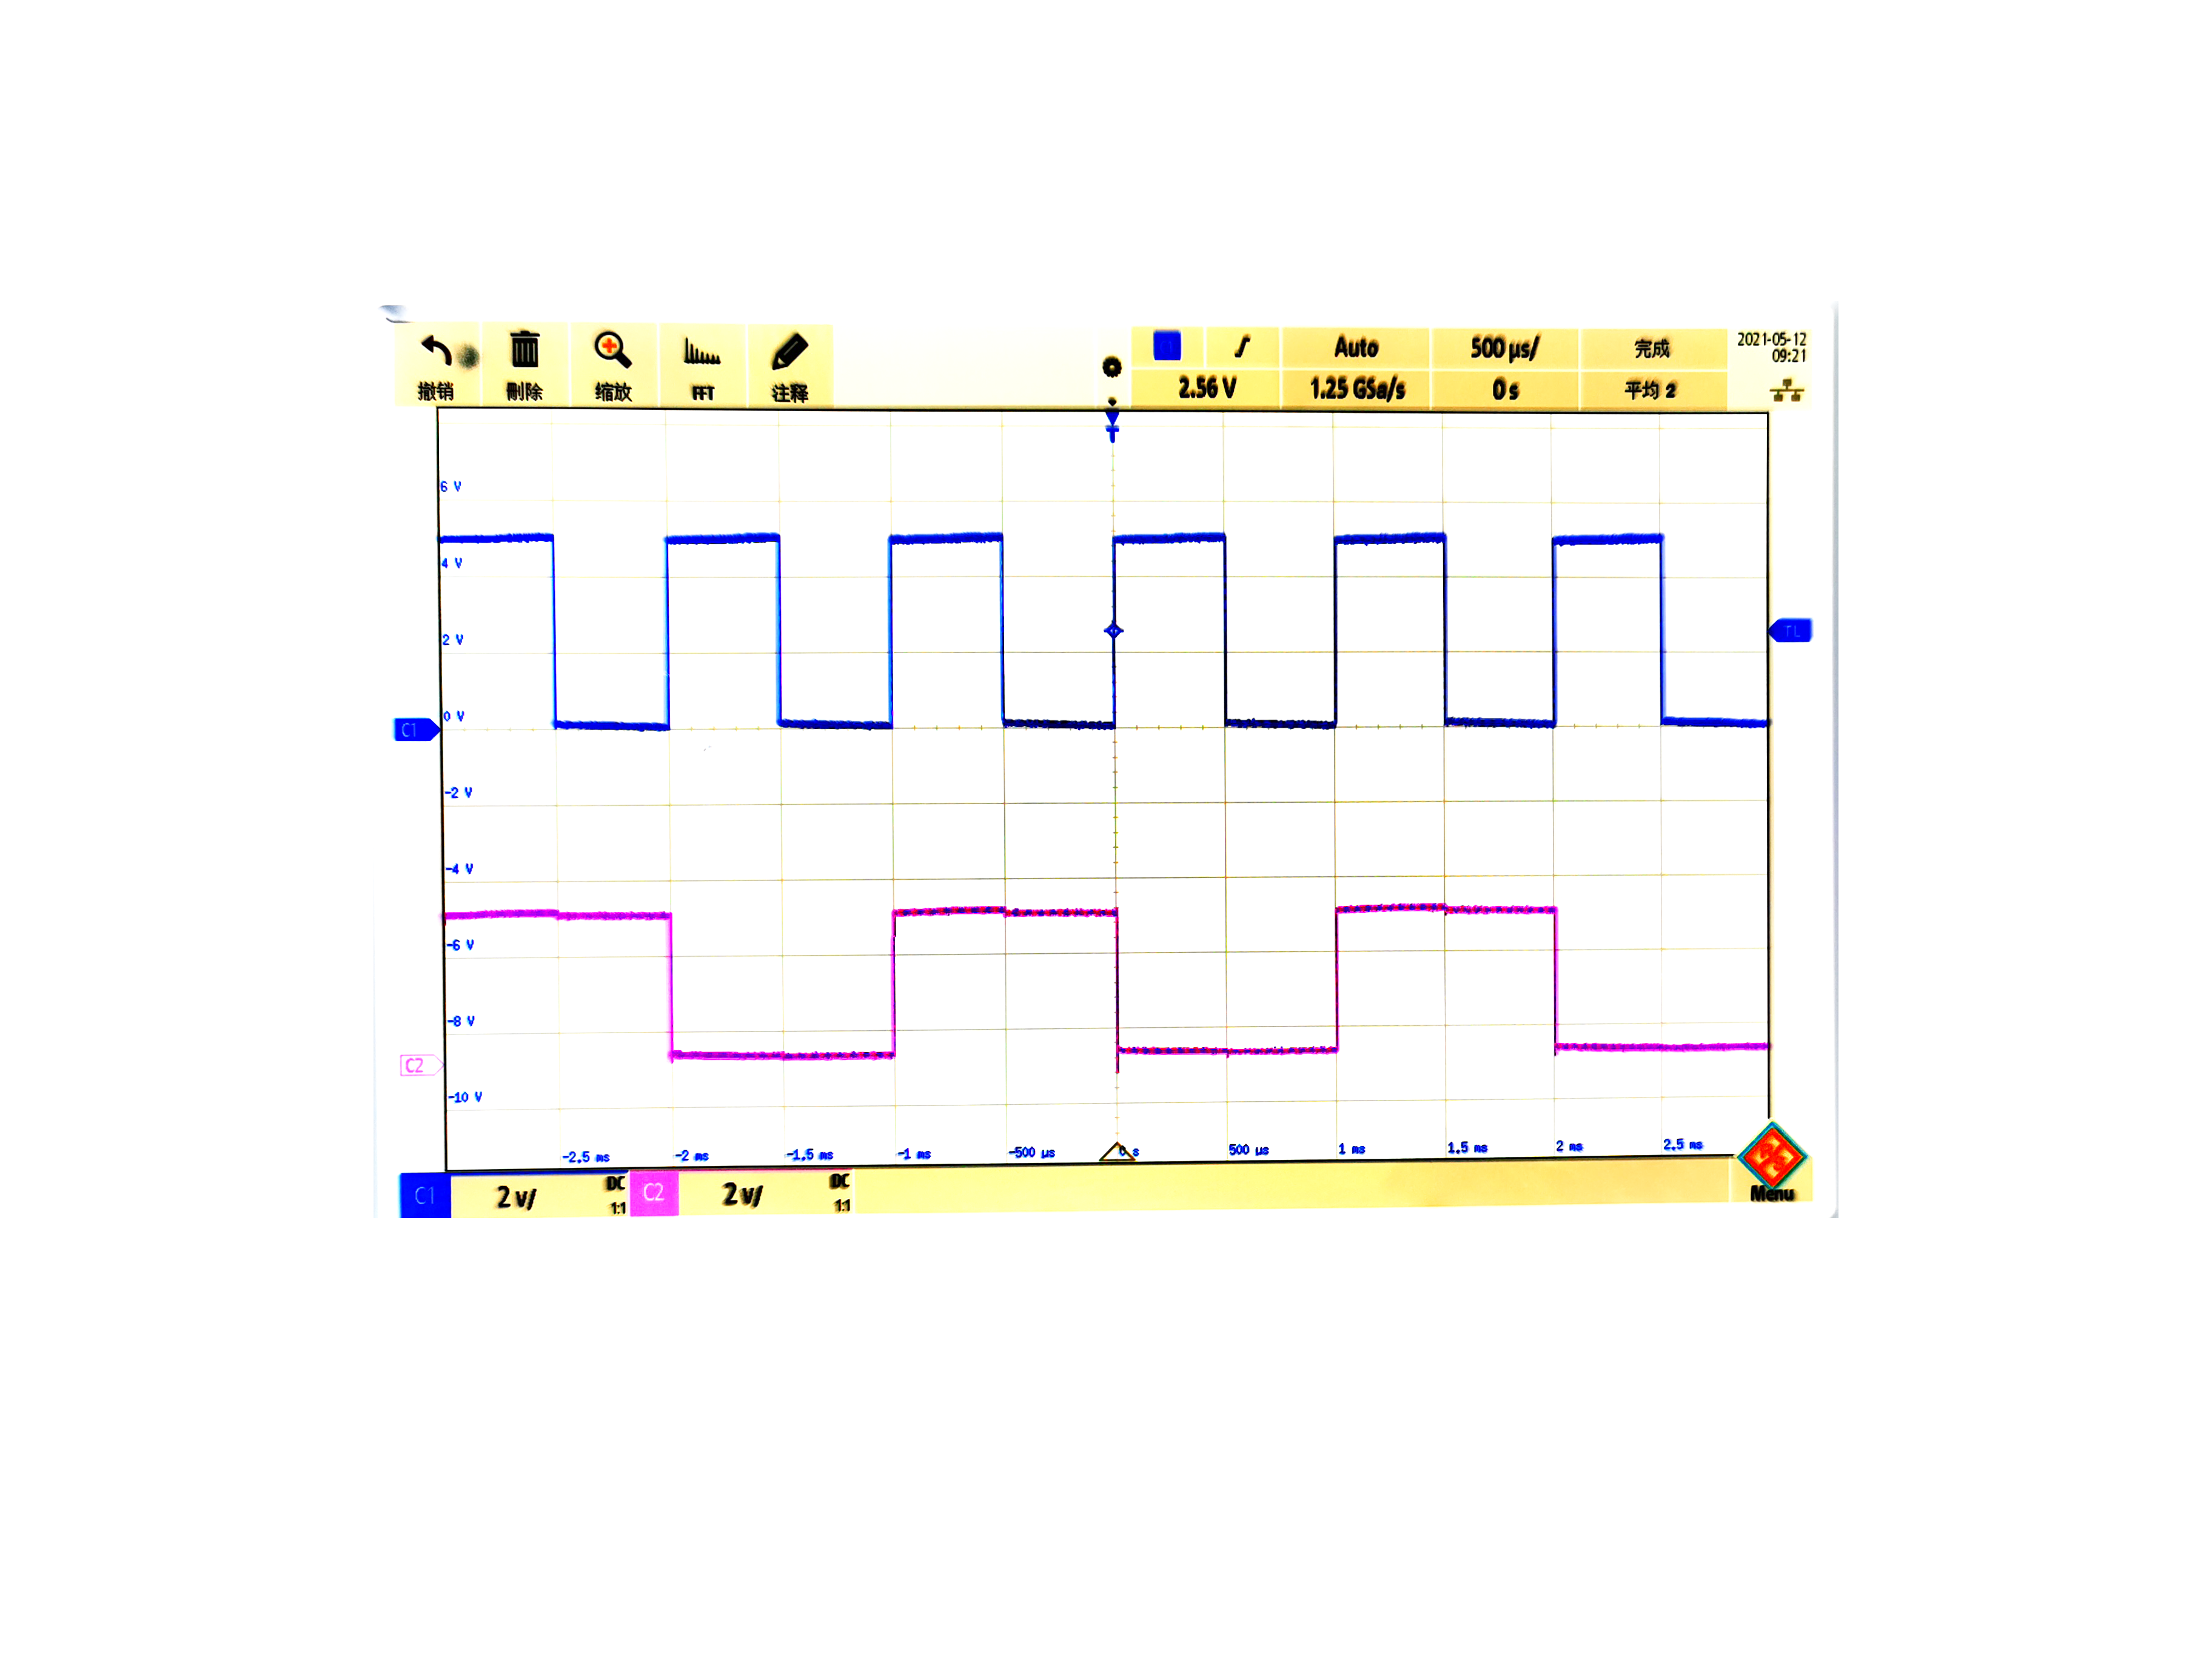
\includegraphics[width=3.3in]{H:/电子技术试验/4-20/4-20-10.png}   
    \caption{$N_o$}   
    \label{fig:side:b}   
  \end{minipage}   
\end{figure}
\newpage
\subsection{竞争与冒险现象}
\begin{figure}[h]
  \begin{minipage}[t]{0.5\linewidth} % 如果一行放2个图,用0.5,如果3个图,用0.33  
    \centering   
    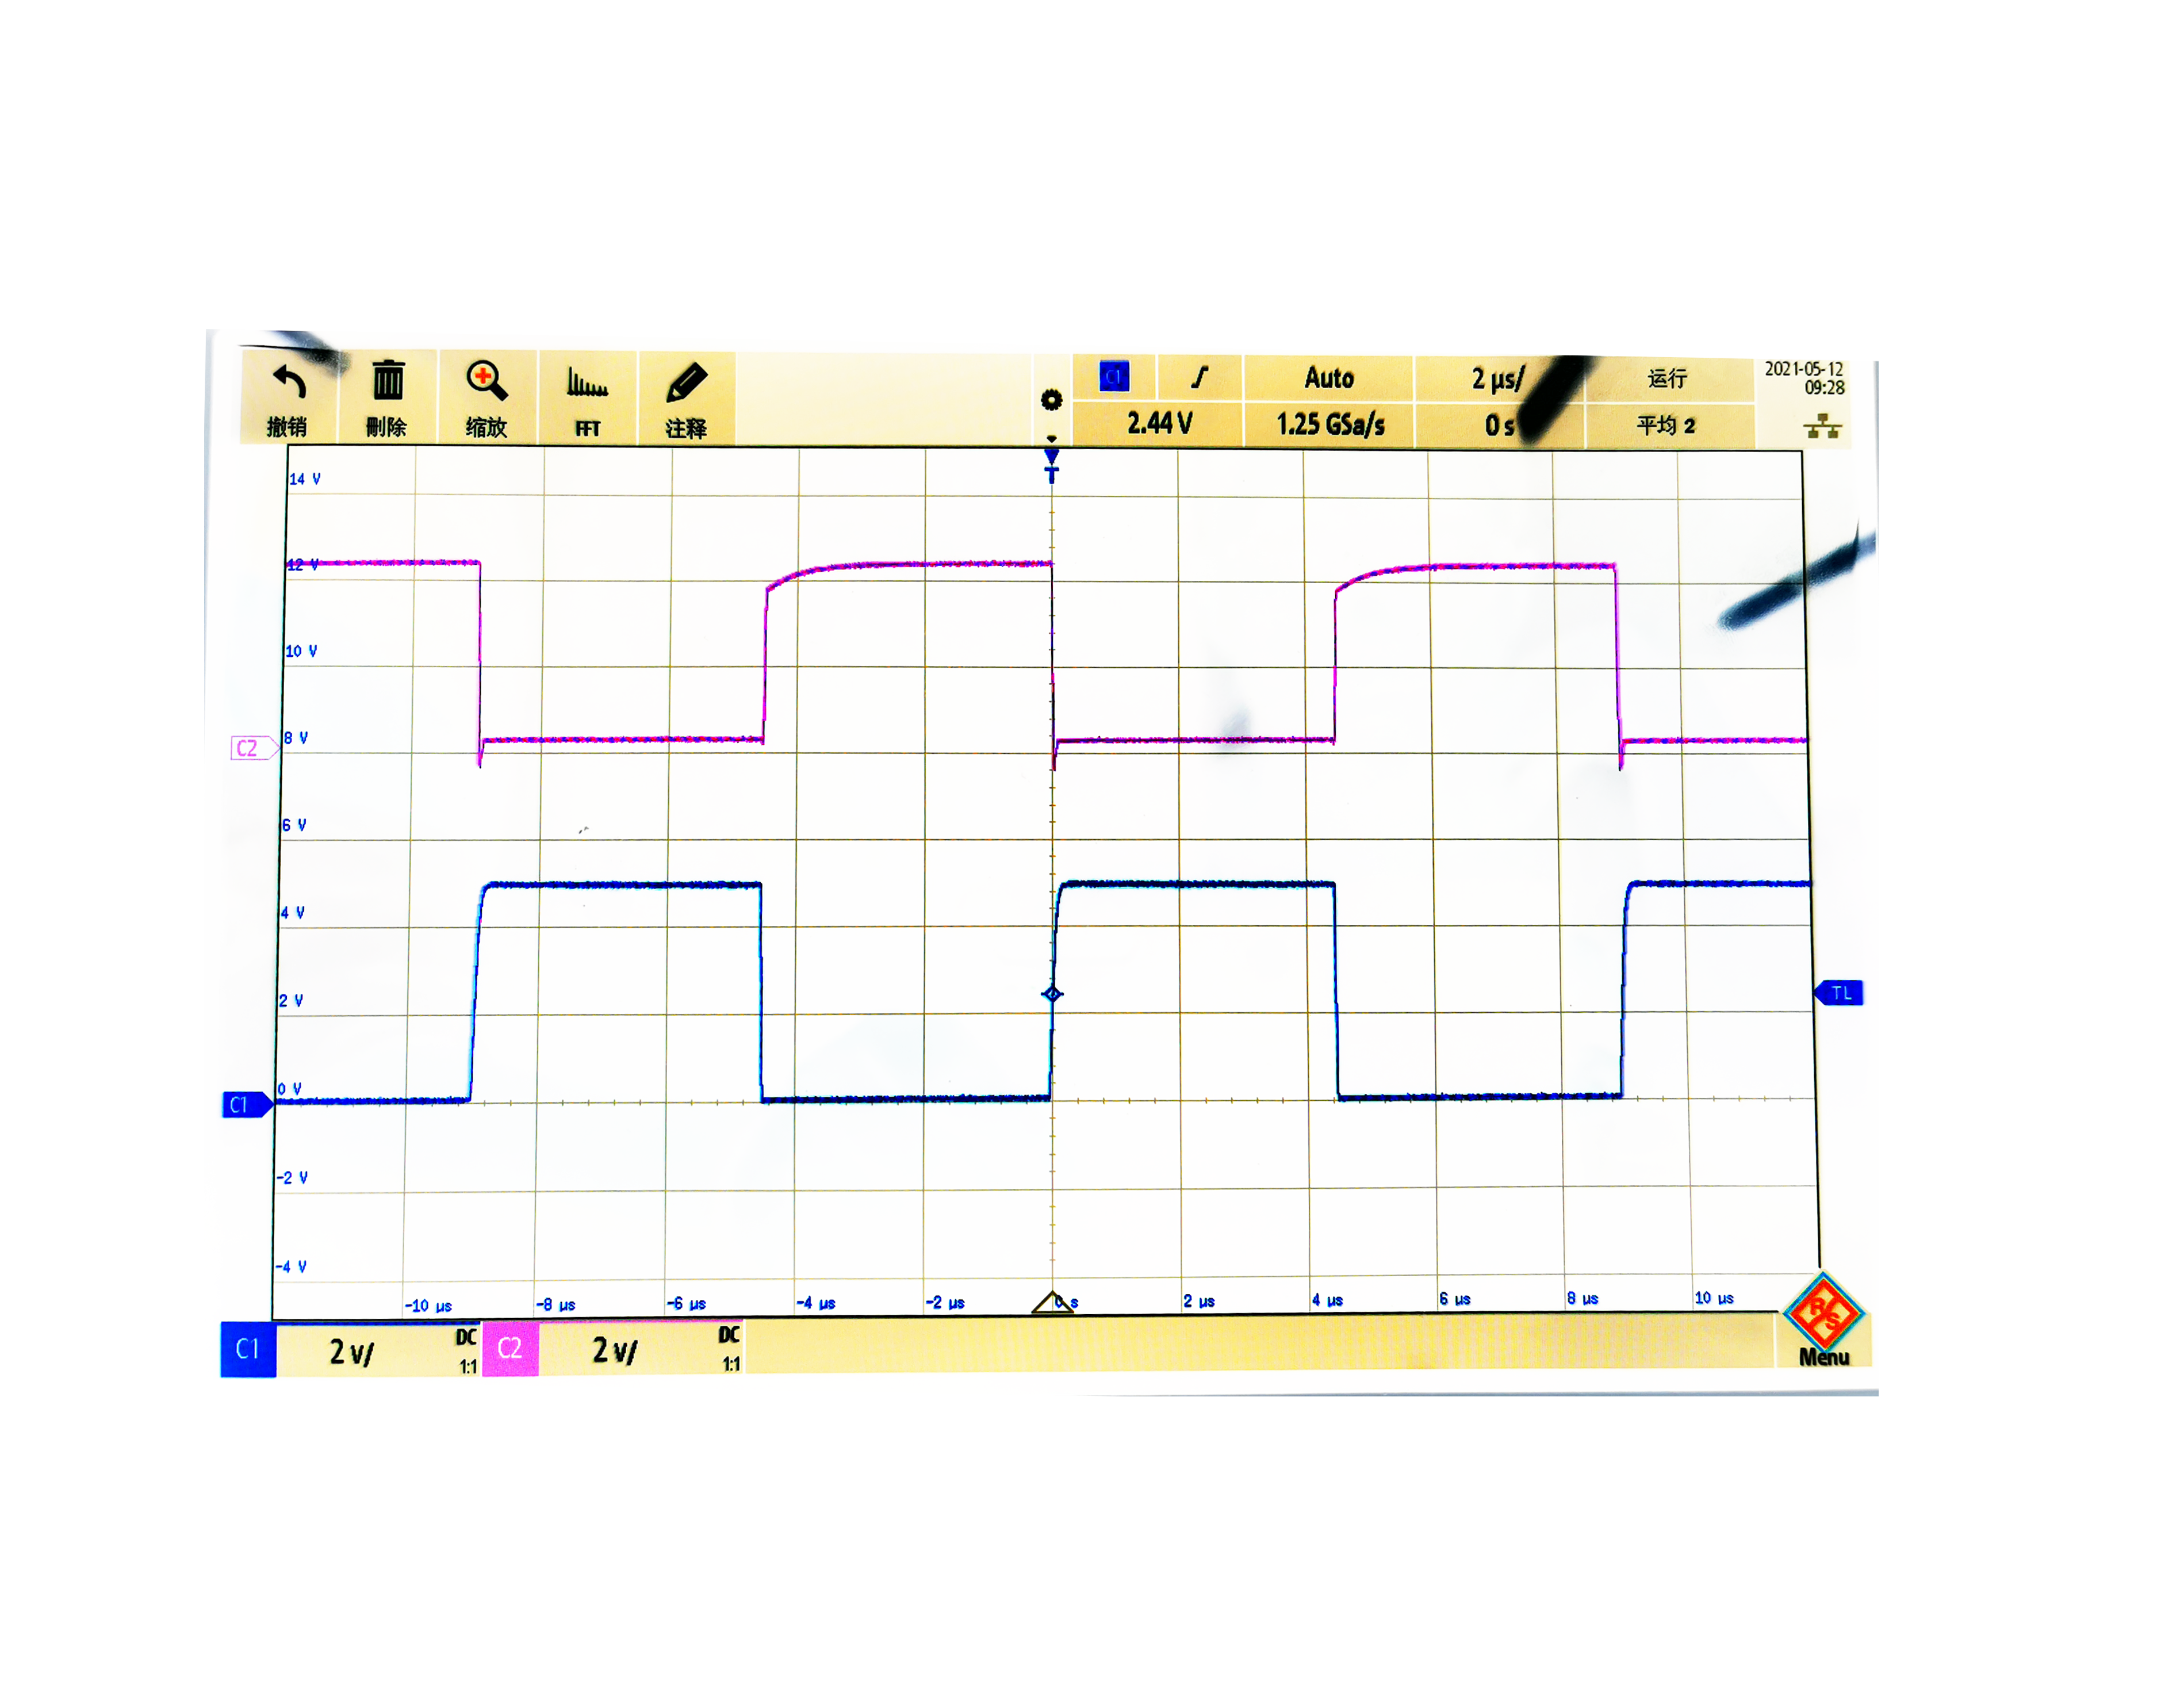
\includegraphics[width=3.3in]{H:/电子技术试验/4-20/4-20-11.png}   
    \caption{$I_{EH}$}   
    \label{fig:side:a}   
  \end{minipage}%   
  \begin{minipage}[t]{0.5\linewidth}   
    \centering   
    \includegraphics[width=3.1in]{H:/电子技术试验/4-20/4-20-13.png}   
    \caption{$N_o$}   
    \label{fig:side:b}   
  \end{minipage}   
\end{figure}

\begin{figure}[h]
  \begin{minipage}[t]{0.5\linewidth} % 如果一行放2个图,用0.5,如果3个图,用0.33  
    \centering   
    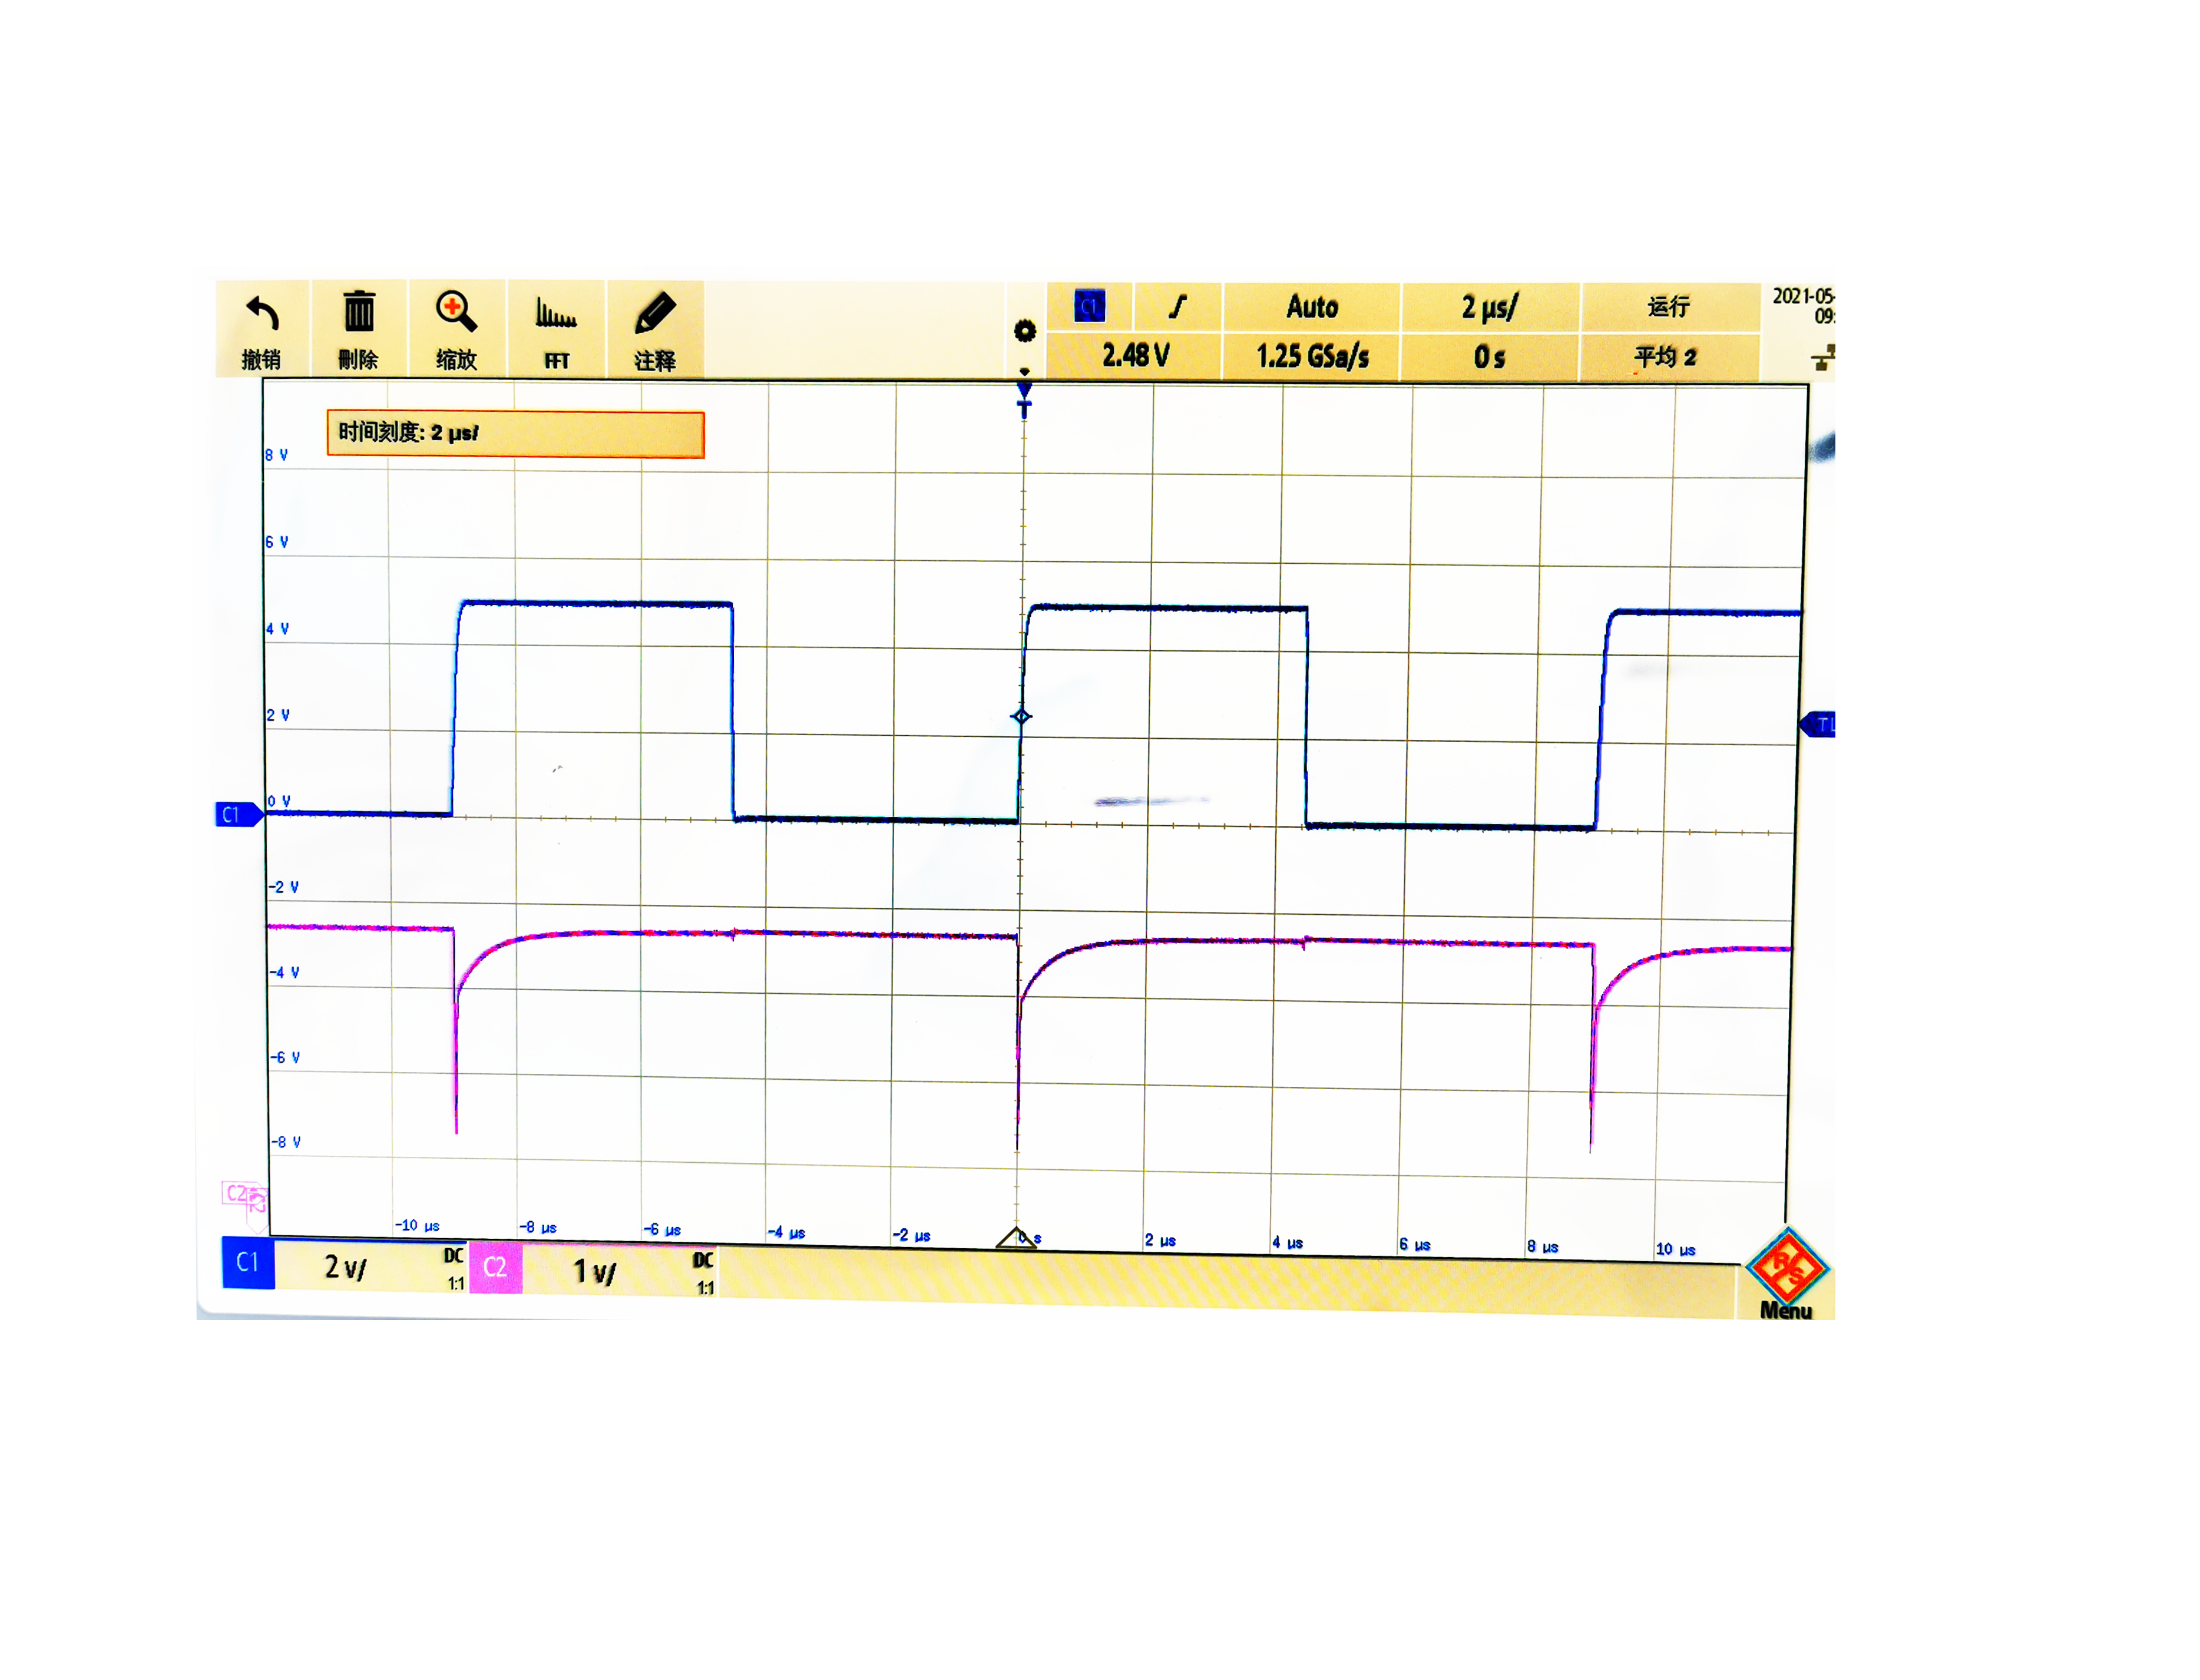
\includegraphics[width=3.3in]{H:/电子技术试验/4-20/4-20-12.png}   
    \caption{$I_{EH}$}   
    \label{fig:side:a}   
  \end{minipage}%   
  \begin{minipage}[t]{0.5\linewidth}   
    \centering   
    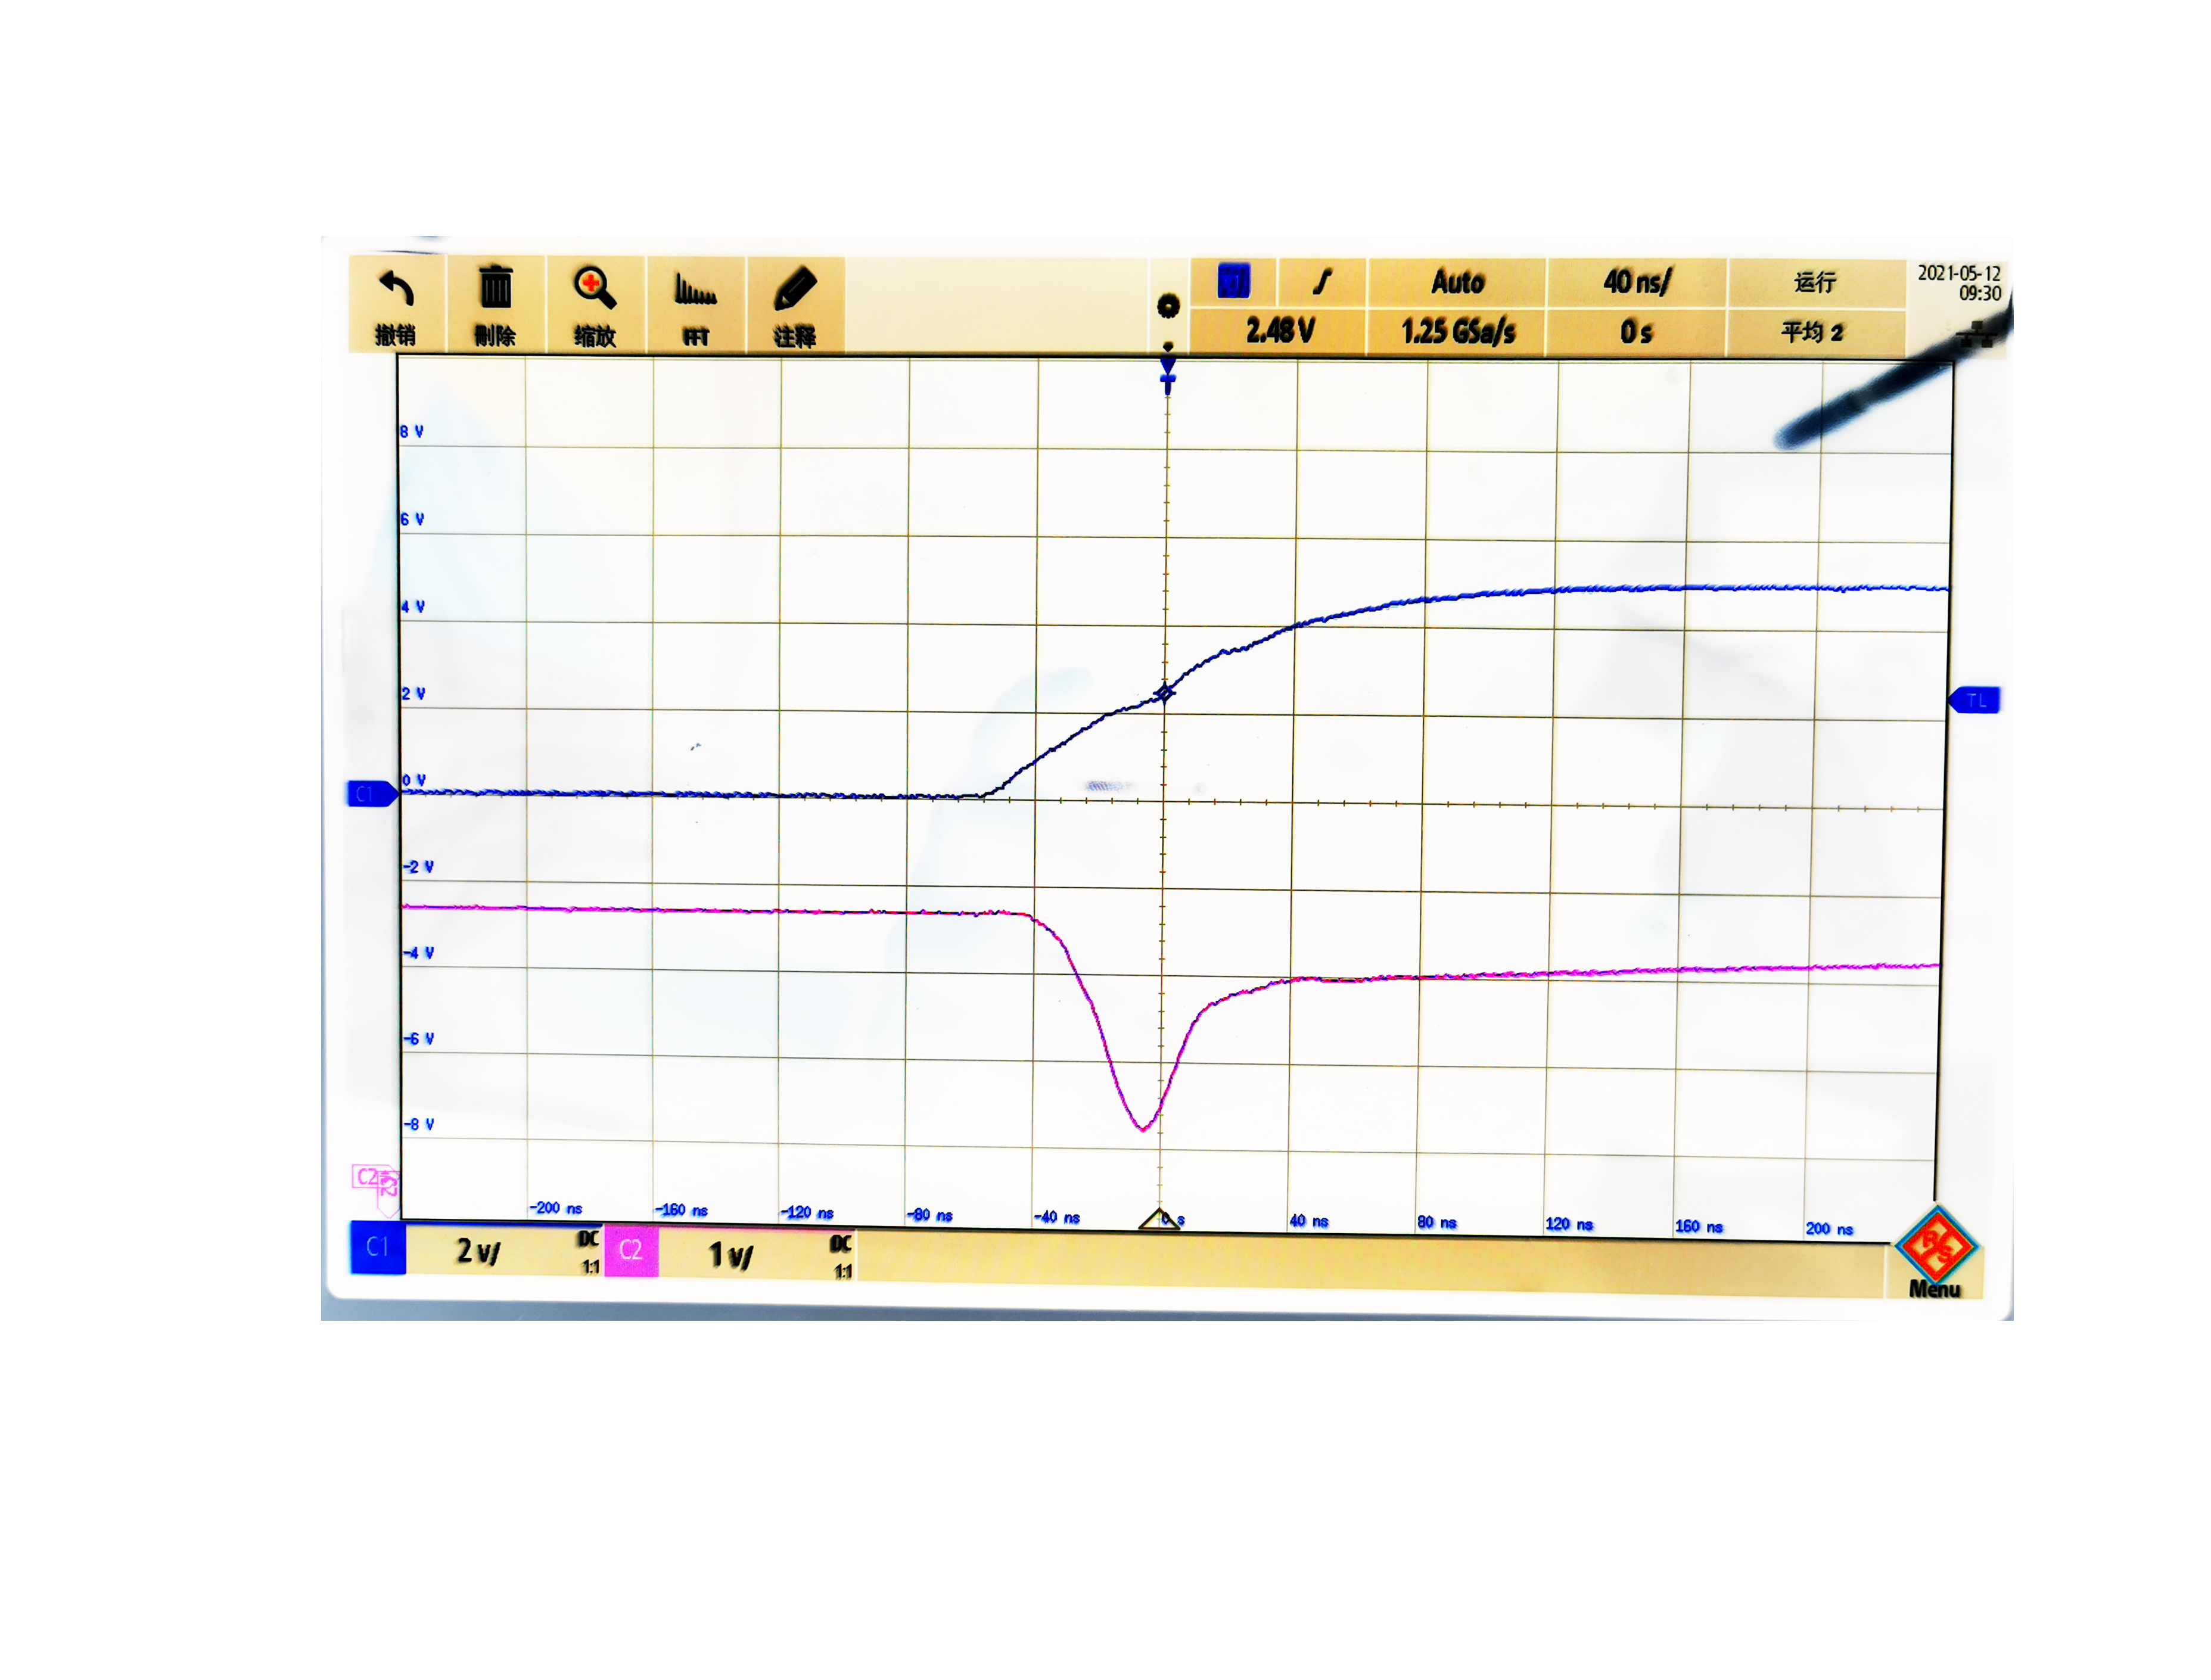
\includegraphics[width=3.3in]{H:/电子技术试验/4-20/4-20-14.png}   
    \caption{$N_o$}   
    \label{fig:side:b}   
  \end{minipage}   
\end{figure}
  
  \newpage
\section{结论}
双稳态触发器具有两个互补的输出端Q和Q',触发器正常工作时,Q与Q'的逻辑电平总是互补,即一个为"0"时另一个一定是"1"。
RS触发器具有两个开关量特性的激励输入端R和S,R的有效电平使触发器复位(Reset),Q="0";S的有效电平使触发器置位(Set),Q="1",所以称为Reset Set 触发器。当激励 S为有效电平时,输出 Q 立即置位为"1",而激励 R 为有效电平时,输出 Q 复位为
"0",两者都为无效电平时,输 出保持原来的状态不变。\par
JK 触发器具有两个激励输入端 J 和 K,其特性
方程为∶$Q_{n+1}=JQ_n'+K'Q_n$。在有效时钟脉冲触发时,
可以实现"同步置位"、"同步复位"、"状态不变"、"状
态变反"四种功能。同时还可以实现分频功能。
\par 
由于电路的设计,在信号传输过程中会产生时间差,会导致竞争冒险现象,即极短时间内,输出信号出现毛刺。


\section{思考}
如果用逻辑开关产生 CP的上升沿或下降沿,可能会出现什么问题?\par
产生信号上升沿和下降沿不明确。
\newpage

\end{document}